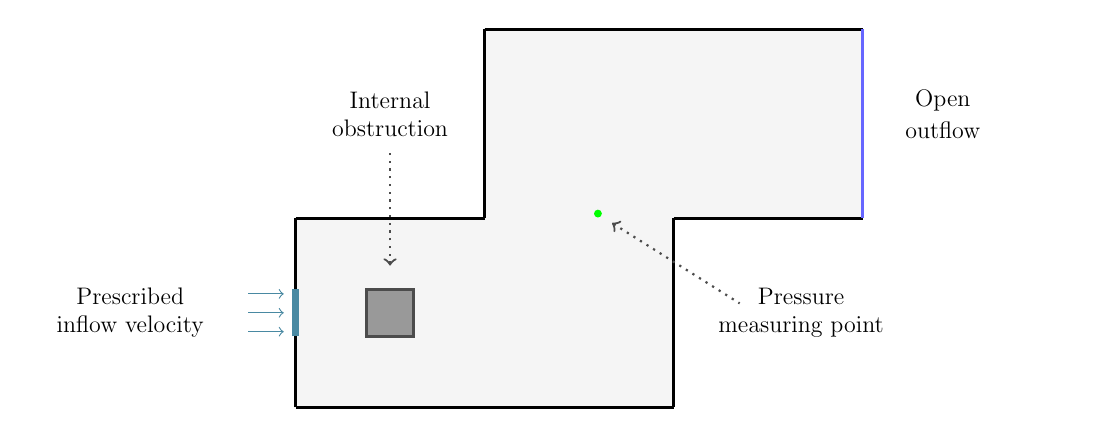
\begin{tikzpicture}
[
scale=0.6,
every node/.style ={scale=0.6},
Background/.style={rectangle,draw=black!04,fill=black!04, thin, minimum size = 4 cm},
Obstruction/.style={rectangle,draw=black!70,fill=black!40, very thick, minimum size=1cm},
Finegrid/.style={step=0.5cm,gray,very thin},
Thickline/.style={-,draw=black!100,fill=black!02, very thick},
Thinline/.style={draw=black!100,fill=black!02, very thin},
Inflow/.style={-,draw={rgb,255:red,73;green,137;blue,162},line width=0.8mm},
Inarrow/.style={->,draw={rgb,255:red,73;green,137;blue,162},thin},
Outflow/.style={-,draw=blue!60,very thick},
Ball/.style={circle, draw=black!40, fill=red!20, thin, minimum size=3.5mm},
Circle/.style={circle,draw=black!40,fill=black!06,thin,minimum size=35.5mm},
Rectangle/.style={rectangle,draw=black!10,fill=white,inner xsep=0pt, inner ysep=0pt,},
Box/.style = {very thin, rectangle, inner xsep=10pt, inner ysep=10pt,},
%Device/.style={fill={rgb,255:red,192;green,58;blue,10}, draw={rgb,255:red,192;green,58;blue,10}},
Device/.style={fill=green, draw=green},
Arrow/.style={thick, dotted, draw=black!70}
]

\node[Background] at (2,2) {};
\node[Background] at (6,2) {};
\node[Background] at (6,6) {};
\node[Background] at (10,6) {};

\node[Obstruction] at (2,2) {};

\draw[Thickline] (0,0)--(8,0);
\draw[Thickline] (4,8)--(12,8);
\draw[Thickline] (0,4)--(4,4);
\draw[Thickline] (8,4)--(12,4);

\draw[Thickline] (0,0)--(0,4);
\draw[Thickline] (4,8)--(12,8);
\draw[Thickline] (4,4)--(4,8);
\draw[Thickline] (8,0)--(8,4);
\draw[Thickline] (12,4)--(12,8);

\draw[Inflow]   (0,1.5)--(0,2.5);
\draw[Inarrow]  (-1,1.6)--(-0.25,1.6);
\draw[Inarrow]  (-1,2.0)--(-0.25,2.0);
\draw[Inarrow]  (-1,2.4)--(-0.25,2.4);
\draw[Outflow]  (12,4)--(12,8);

\draw[Device] (6.4,4.1) circle (2pt);
\draw [<-, Arrow] (6.7,3.9) -- (9.4,2.2);
\draw [<-, Arrow] (2.0,3.0) -- (2.0,5.4);
\node [Box] (Box) at (-3.5,2.0)  {\begin{minipage}{0.3\textwidth}\centering{\Large Prescribed\\[0.8ex] inflow velocity}\end{minipage}};
\node [Box] (Box) at (13.7,6.2){\begin{minipage}{0.4\textwidth}\centering{\Large Open \\[0.8ex] outflow}\end{minipage}};
\node [Box] (Box) at (2.0,6.2)  {\begin{minipage}{0.4\textwidth}\centering{\Large Internal \\[0.8ex] obstruction}\end{minipage}};
\node [Box] (Box) at (10.7,2.0){\begin{minipage}{0.4\textwidth}\centering{\Large Pressure  \\[0.8ex] measuring point}\end{minipage}};
\end{tikzpicture}

